%===============================
\section{Inserção}
%===============================
A dupla começou o desenvolvimento da árvore pela inserção de elementos, pois já tinhamos a base no livro indicado pela professora. A implementação foi básicamente transformar aquele pseudo-código no nosso código C. Tivemos alguns problemas em relação ao tamanho dos vetores, já que no pseudo-código eles começavam pelo número 1 e na linguagem C começa-se pelo 0.
\par Nas primeiras versões do nosso código, alguns problemas foram apresentados ao dividir um nó, não verificavamos se o lugar apropriado para o novo elemento era o nó esquerdo ou direito, por consequência disso, todo novo elemento automaticamente ia para o nó esquerdo, demoramos para localizar o erro, porém após identificado, a solução foi elementar.  

\begin{figure}[!h]
\centering
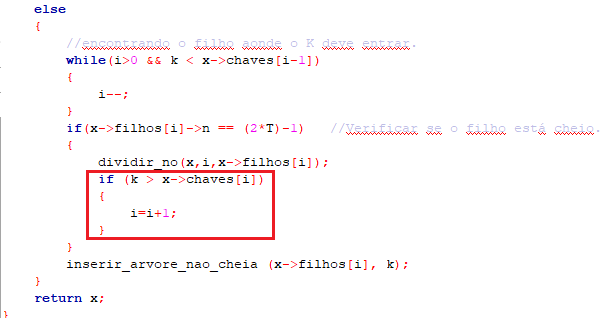
\includegraphics[width=6in]{relatorio/imagens/imgIfInsercao.png}
\end{figure}